\justify
\section{Pregunta 11}

\begin{table}[h]
	\begin{center}
		\caption{Intervalos de confianza al 95\% sobre la influencia de los padres en la elecci�n de carrera}
		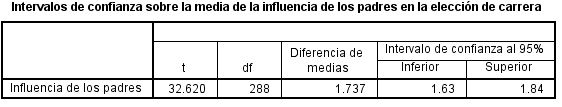
\includegraphics[scale=.50]{IDCP11.JPG}
	\end{center}
\end{table}

En la pregunta 11 se le solicit� informaci�n al encuestado sobre que tanto consideraba que sus padres hab�an influenciado la elecci�n de su carrera, al analizar esta variable se obtuvo que la media poblacional, se encontraba con el 95\% de confianza entre los valores de 1.63 y 1.84, con esto se concluye que la mayor�a de los estudiantes de la Universidad del Valle fueron poco influenciados por sus padres.
\section{Pregunta 12}

\begin{table}[h]
	\begin{center}
		\caption{Intervalos de confianza al 95\% sobre la proporci�n de elecci�n de carrera si el estudiante no hubiera sido influenciado}
		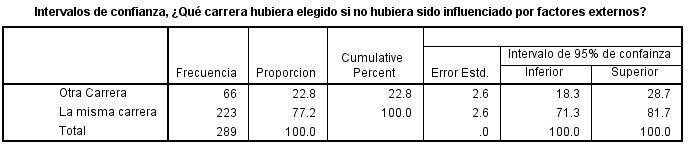
\includegraphics[scale=.50]{IDCP12.JPG}
	\end{center}
\end{table}

Como se puede observar en la pregunta 12 se buscaba encontrar la proporci�n de estudiantes que, considerando que no hubiesen sido influenciados por factores externos si es que hubieron, que carrera hubieran elegido. Los resultados reflejaron que con el 95\% de confianza la proporci�n de personas que hubieran seguido en su misma carrera est� entre 71.3\% y 81.7\%, mientras que la proporci�n de personas que hubieran elegido la misma carrera, se encuentra entre 18.3\% y 28.7\%.

Gracias a estos resultados se puede ver en los intervalos de confianza que la mayor�a de los estudiantes de la Universidad del Valle est�n dispuestos a seguir en la carrera en la que se encuentran.

\section{Pregunta 13}

\begin{table}[h]
	\begin{center}
		\caption{Intervalos de confianza al 95\% de la proporci�n de intenci�n de cambio de carrera universitaria }
		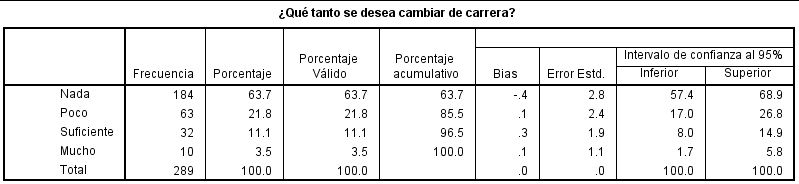
\includegraphics[scale=.50]{IDCP13.JPG}
	\end{center}
\end{table}

En la pregunta 13 se buscaba cuantificar la intenci�n del estudiante encuestado de cambiarse de carrera. Seg�n la muestra obtenida, se encontr� que la intenci�n de no realizar ning�n cambio de carrera, se encontraba presente con el 95\% de confianza entre el 57.4\% y 68.9\% de los encuestados. Respecto a las intenciones de un convencimiento peque�o de cambio de carrera, se encontr� que la proporci�n se encontraba entre el 17\% y 26.8\%. En cuanto a la proporci�n de estudiantes que consideraban que sus intenciones eran las suficientes para realizar un cambio de carrera esta entre 8.0\% y 14.9\%. Por �ltimo la proporci�n de  estudiantes que estaban decididos a realizar un cambio de carrera se encontraba entre 1.7\% y 5.8\%.

Con estos resultados se puede concluir que la mayor�a de los estudiantes de la Universidad del Valle, se encuentran dispuestos a continuar con su carrera ya que la proporci�n de personas que considera que no es beneficioso realizar un cambio de carrera es dominante en la muestra.